\documentclass[11pt,a4paper]{article}

\usepackage[utf8]{inputenc}
\usepackage[T1]{fontenc}
\usepackage[spanish,es-noquoting]{babel}
\usepackage{lmodern}
\usepackage[margin=2.5cm]{geometry}
\usepackage{graphicx}
\usepackage{array}
\usepackage{tabularx}
\usepackage{xltabular}
\usepackage[table]{xcolor}
\usepackage{cite}
\usepackage{hyperref}

\definecolor{verdeuteq}{RGB}{27,117,5}
\newcolumntype{L}{>{\raggedright\arraybackslash}X}
\renewcommand{\arraystretch}{1.3}

\begin{document}

% Portada. Si el docente comparte la plantilla oficial de la UTEQ, se reemplaza esta.
\begin{titlepage}
\centering

\includegraphics[width=0.75\textwidth]{figuras/logo_uteq.png}\par
\vspace{1.5cm}
{\large Facultad de Ciencias de la Computación\par}
{\large Carrera de Ingeniería de Software\par}
\vspace{1.5cm}
{\Large\bfseries PE1 -- Unidad 1\par}
\vspace{0.4cm}
{\Large Ingeniería de Requisitos y Proceso de Requisitos\par}
\vspace{1.5cm}
{\large Integrantes:\par}
Aldas Zambrano Alan Andrés\par
Naranjo Flores Anderson Jeampiere\par
Yépez Guagua Luis Antonio\par
\vspace{1.5cm}
Asignatura: Ingeniería de Requerimientos (ISR-401)\par
4.º nivel, paralelo A\par
Docente: Ing. Gleiston Cicerón Guerrero Ulloa, PhD\par
\vfill
Quevedo -- Ecuador\par
2026
\end{titlepage}


\tableofcontents
\clearpage

% La guía (Paso 6b) pide: secc. 0 (PFC), secc. 2 (fundamento), secc. 3 (artefactos).
\setcounter{section}{-1}
% Paso 1 (Alan). Sección 0 del documento.
\section{Sistema del Proyecto Fin de Curso}

\subsection{Roles del equipo}
% Paso 1 a) y b): rol, nombre completo, cédula y correo institucional de cada integrante.
% La guía tiene 5 roles para 3 integrantes: el grupo decide cómo se reparten.

\begin{center}
\small
\begin{tabularx}{\textwidth}{|>{\raggedright\arraybackslash}p{3.5cm}|L|>{\raggedright\arraybackslash}p{2.3cm}|>{\raggedright\arraybackslash}p{4.2cm}|}
\hline
\rowcolor{verdeuteq}\textcolor{white}{\textbf{Rol}} & \textcolor{white}{\textbf{Nombre completo}} & \textcolor{white}{\textbf{Cédula}} & \textcolor{white}{\textbf{Correo institucional}} \\ \hline
 & & & \\ \hline
 & & & \\ \hline
 & & & \\ \hline
\end{tabularx}
\end{center}

\subsection{Descripción del sistema}
% Paso 1 c): máximo 150 palabras. Nombre, problema que resuelve, usuarios principales y contexto organizacional.

UteqFit-AI es un sistema para el gimnasio de la UTEQ, que es gratuito. Se supone que actualmente el registro de los usuarios se hace de forma manual, lo que dificultaría controlar quién ocupa los cupos y quién dejó de asistir. Lo usarían los estudiantes, los encargados del gimnasio y Bienestar Universitario. Además, el sistema usaría inteligencia artificial para sugerir la rutina de cada usuario, y esa rutina la aprobaría un entrenador antes de asignarla, si el gimnasio cuenta con uno.

\subsection{Stakeholders y matriz poder/interés}
% Paso 1 d): los 5 stakeholders principales clasificados con la matriz poder/interés del PMBOK 7.a ed.

Los stakeholders se clasificaron con la matriz poder/interés del PMBOK~\cite{pmbok7}.

\begin{center}
\small
\begin{tabularx}{\textwidth}{|>{\raggedright\arraybackslash}p{3.5cm}|>{\centering\arraybackslash}p{1.6cm}|>{\centering\arraybackslash}p{1.6cm}|L|}
\hline
\rowcolor{verdeuteq}\textcolor{white}{\textbf{Stakeholder}} & \textcolor{white}{\textbf{Poder}} & \textcolor{white}{\textbf{Interés}} & \textcolor{white}{\textbf{Estrategia}} \\ \hline
Estudiantes & Bajo & Alto & Mantener informados \\ \hline
Responsable del gimnasio & Alto & Alto & Gestionar de cerca \\ \hline
Encargado de turno & Bajo & Alto & Mantener informado \\ \hline
Bienestar Universitario & Alto & Bajo & Mantener satisfecho \\ \hline
Entrenador (si existe) & Bajo & Alto & Mantener informado \\ \hline
\end{tabularx}
\end{center}

\subsection{Tipo de sistema}
% Paso 1 e): a qué tipo de sistema pertenece (según la secc. 2.5) y por qué.


\setcounter{section}{1}
\section{Fundamento teórico}
\subsection{Ingeniería de requisitos}

\subsubsection{Definición y alcance}

La ingeniería de requisitos reúne las actividades que permiten
identificar, analizar, especificar, validar y gestionar las necesidades
y restricciones de un sistema a lo largo de su ciclo de
vida~\cite{ieee29148,pohl2025,swebok2024}.

Una necesidad expresa el problema que un interesado quiere resolver.
Para convertirla en un requisito, el equipo debe aclarar qué
comportamiento espera del sistema y en qué condiciones debe ocurrir.
Registrar la fuente de esa decisión permite revisarla cuando el equipo
encuentra una excepción o cambia el alcance del
proyecto~\cite{ieee29148,pohl2025}.

\textbf{Ejemplo en UteqFit-AI.}
La necesidad de conocer la ocupación del gimnasio se traduce en
RF-06, que pide mostrar cuántos estudiantes tienen una entrada
registrada sin su salida correspondiente. Para revisar ese requisito,
se puede preparar un caso con tres entradas y dos salidas asociadas.
El resultado esperado es que el sistema muestre una persona dentro.

\subsubsection{Actores del proceso}

En ingeniería de requisitos, los interesados son personas u
organizaciones que tienen interés en el sistema o pueden verse
afectadas por él. Sus necesidades y restricciones aportan información
para definir lo que el sistema debe hacer~\cite{ieee29148,pohl2025}.

El ingeniero de requisitos organiza las consultas y documenta las
decisiones. El cliente o responsable del proyecto confirma las
prioridades y los usuarios explican cómo realizan las operaciones
cotidianas. El desarrollador aporta información sobre la viabilidad
técnica y ayuda a aclarar las condiciones necesarias para implementar
y comprobar los requisitos~\cite{pohl2025,swebok2024}.

\textbf{Ejemplo en UteqFit-AI.}
Para revisar RF-06, el equipo del PFC puede preparar los casos de
prueba y consultar al encargado de turno sobre qué sucede cuando
un estudiante se va sin registrar su salida. El responsable del
gimnasio puede decidir cómo debe tratarse ese caso. El desarrollador
puede valorar qué información haría falta para corregir el registro
y conservar el historial de la operación.
\subsection{Proceso de ingeniería de requisitos}

\subsubsection{Actividades centrales del marco de Pohl}

Pohl distingue tres actividades centrales: la elicitación, que permite
obtener información de las fuentes, la documentación, que registra
los requisitos y sus decisiones, y la negociación, que busca resolver
diferencias entre los interesados~\cite{pohl2025}.

Durante la elicitación, el equipo puede consultar a quienes realizan
una tarea y revisar los documentos que usan. La documentación
permite conservar qué necesidad se identificó y de dónde proviene.
Si dos actores esperan resultados distintos, la negociación ayuda
a decidir qué se incorpora al alcance y a registrar el motivo de
esa decisión~\cite{pohl2025,swebok2024}.

\textbf{Ejemplo en UteqFit-AI.}
Para revisar RI-01, el equipo puede solicitar a Bienestar
Universitario una descripción del listado de estudiantes habilitados
y consultar al encargado sobre su uso. Después puede documentar
cuándo se entrega el listado y qué información necesita la
importación. Si se pide una actualización distinta a la prevista
por período académico, el equipo tendría que acordar quién la
autoriza y cómo se entrega.

\subsubsection{Actividades transversales}

En el marco de Pohl, la validación comprueba si los requisitos
representan las necesidades de los interesados. La gestión de
requisitos mantiene su identificación, sus relaciones y su historial
de cambios durante el proyecto~\cite{pohl2025,ieee29148}.

La validación permite revisar un borrador con quienes conocen la
operación del gimnasio. Si esa revisión revela un caso omitido,
el equipo puede actualizar el requisito y su criterio de aceptación.
La gestión ayuda a conservar la relación entre el cambio, la fuente
que lo motivó y los requisitos que dependen de él~\cite{pohl2025,swebok2024}.

\textbf{Ejemplo en UteqFit-AI.}
Para revisar la importación del listado, se pueden preparar dos
casos con datos ficticios: un estudiante que figura como habilitado
y otro que no aparece en el archivo. Bienestar Universitario y el
encargado de turno pueden revisar el resultado esperado para cada
caso. Si acuerdan un tratamiento especial para las discrepancias,
el equipo puede registrar la decisión en RI-01 y revisar su
compatibilidad con RR-01.

\subsubsection{Secuencia de trabajo aplicada al PFC}

SWEBOK organiza el trabajo con requisitos en actividades que incluyen
elicitación, análisis, especificación y validación. Estas actividades
pueden repetirse cuando aparece información que obliga a modificar
un requisito~\cite{swebok2024,ieee29148}.

La elicitación permite identificar qué necesita cada actor y qué
información puede aportar. En el análisis, el equipo contrasta esa
información con el alcance del sistema y revisa posibles
contradicciones. En la especificación, convierte las decisiones
en enunciados identificables y verificables. En la validación,
los interesados revisan si los enunciados y los casos de aceptación
reflejan la operación esperada~\cite{swebok2024,ieee29148}.

\textbf{Ejemplo en UteqFit-AI.}
Para el control de ocupación, la secuencia propuesta comienza
con una consulta al encargado sobre el registro de entradas y
salidas. Sigue con el análisis de qué cuenta como visita abierta
y con la especificación de RF-01, RF-02 y RF-06. La revisión
con el responsable del gimnasio puede utilizar casos de entrada,
salida y visita sin cerrar. Como evidencia de aplicación, el
equipo puede adjuntar la nota de la consulta, la versión de los
requisitos revisada y el registro de los resultados cuando se
realice la validación.
% Paso 3 (Luis). Sección 2.3. Falta el título exacto de la guía.
% Cada concepto: (i) definición formal con cita, (ii) explicación propia de mínimo 3 oraciones,
% (iii) ejemplo concreto del gimnasio de la UTEQ.
% Aquí van los tipos de requisito que usa la tabla de la sección 3 (Paso 4 a).
\subsection{}

% Aporte de Luis: sección 2.4. Título de trabajo no confirmado por el docente.
% Las propiedades se presentan conforme al enfoque de ISO/IEC/IEEE 29148:2018.
\subsection{Propiedades de calidad de los requisitos}
\label{sec:calidad-requisitos}

Un requisito bien escrito no garantiza por sí solo que el proyecto resolverá el problema correcto. Es necesario examinar cada enunciado y, después, revisar el conjunto para detectar ausencias, contradicciones y duplicaciones~\cite{ieee29148}. En UteqFit-AI, esta evaluación se aplicaría primero a la tabla preliminar de requisitos del equipo y posteriormente a las versiones acordadas con los actores del gimnasio.

\subsubsection{Necesidad y pertinencia}
Un requisito es necesario cuando responde a una necesidad comprobable o a una obligación que deba atender el sistema~\cite{ieee29148}. Incluir funciones por simple interés tecnológico aumenta el trabajo sin demostrar su beneficio. Para decidir si se conserva una idea, el equipo debe preguntar quién la necesita y qué problema evita. Por ejemplo, recomendar rutinas mediante IA es una propuesta opcional del PFC; su prioridad depende de confirmar que existe una persona autorizada para revisarlas y que los estudiantes realmente las consideran útiles.

\subsubsection{Claridad y ausencia de ambigüedad}
Un requisito debe permitir una interpretación consistente entre quien lo solicita, quien lo desarrolla y quien lo verifica~\cite{ieee29148}. Expresiones como ``fácil de usar'' o ``notificar pronto'' pueden producir resultados diferentes según la persona. Para mejorarlas hay que precisar actor, situación y resultado observable. En UteqFit-AI, ``mostrar las asistencias'' se aclara indicando si se muestran al estudiante, al encargado o a Bienestar Universitario y cuál es el intervalo de fechas consultado.

\subsubsection{Completitud y singularidad}
Un requisito completo incluye la información imprescindible para entender qué comportamiento se espera; además, conviene que exprese una sola obligación por enunciado~\cite{ieee29148}. Si mezcla guardar asistencia, enviar alertas y elaborar reportes, una prueba podría aprobar una parte y fallar las otras. La separación también facilita estimar esfuerzos y localizar fallos. En UteqFit-AI sería preferible identificar por separado el registro de entrada, el registro de salida y el cálculo de ocupación actual.

\subsubsection{Factibilidad}
La factibilidad obliga a revisar si el requisito puede implementarse dentro de las restricciones de tiempo, recursos, tecnología y operación~\cite{ieee29148}. Que una función sea atractiva no significa que existan los datos o permisos necesarios para ponerla en marcha. El análisis debe señalar dependencias y alternativas antes de comprometerse a desarrollarla. Para UteqFit-AI, las rutinas sugeridas mediante IA requieren evaluar disponibilidad de datos apropiados, revisión humana y límites de responsabilidad; todavía no corresponde declarar esa capacidad como validada.

\subsubsection{Verificabilidad}
Un requisito verificable permite decidir, mediante un procedimiento definido, si el producto lo cumple o no~\cite{ieee29148}. Es útil establecer condiciones de prueba, datos de entrada y resultado esperado. Los calificativos subjetivos deben sustituirse por observaciones que puedan repetirse. Por ejemplo, para el registro de entrada se puede comprobar que una acción autorizada crea un registro con identificación del estudiante, fecha y hora; para rendimiento se requiere además acordar una carga de prueba y un tiempo máximo.

\subsubsection{Corrección y consistencia}
La corrección se relaciona con representar fielmente la necesidad acordada; la consistencia exige que los requisitos del conjunto no se contradigan~\cite{ieee29148}. Dos enunciados pueden ser claros por separado y aun así establecer reglas incompatibles. Por eso se revisan juntos, idealmente con las partes interesadas autorizadas. En UteqFit-AI se debería comprobar que las reglas de acceso, consulta de historial y tratamiento de datos personales no permitan a un rol visualizar información que le está restringida en otro requisito.

\subsubsection{Trazabilidad}
La trazabilidad mantiene los vínculos entre origen, requisito, decisiones de diseño y evidencias de verificación~\cite{ieee29148}. Es importante porque una modificación en las reglas de uso del gimnasio podría afectar varias funciones. Cada cambio debería permitir identificar qué se modifica, quién lo autorizó y qué pruebas deben repetirse. Como mecanismo propuesto, el equipo puede conservar una matriz con ID, fuente, versión, criterio de aceptación y prueba asociada para cada requisito de UteqFit-AI.

\subsubsection{Conformidad de redacción}
La especificación debe seguir las reglas de presentación acordadas, con identificadores estables y vocabulario uniforme~\cite{ieee29148}. Esto evita que varios integrantes utilicen términos diferentes para la misma persona o función. También facilita revisar los requisitos y actualizar documentos sin perder referencias. En UteqFit-AI se propone mantener ``estudiante'', ``encargado de turno'' y ``responsable del gimnasio'' como roles distintos, mientras no se confirme que alguno comparte responsabilidades.

\subsubsection{Calidad del conjunto de requisitos}
Además de revisar cada enunciado, hay que comprobar que el conjunto sea suficientemente completo, consistente y adecuado para su propósito~\cite{ieee29148}. La tabla podría tener quince requisitos bien redactados y aun así omitir cómo se corrige un registro de asistencia equivocado. También podría contener funciones que no tienen una fuente validada. La revisión colectiva debe señalar expresamente esos vacíos y distinguir los requisitos confirmados de las propuestas todavía pendientes.

% Aporte de Luis: sección 2.5. Título de trabajo, por confirmar con el índice oficial.
\subsection{Tipos de sistemas y ubicación de UteqFit-AI}
\label{sec:tipos-sistemas}

Determinar el tipo de sistema ayuda a reconocer sus fuentes de requisitos, riesgos y condiciones de uso. Una clasificación puede considerar la finalidad de la solución, sus componentes tecnológicos y la forma en que reacciona ante el entorno~\cite{pohl2025,swebok2024}. Los siguientes tipos son útiles para la práctica; no constituyen una taxonomía exclusiva o una enumeración normativa de ISO/IEC/IEEE 29148.

\subsubsection{Sistema de información}
Un sistema de información organiza datos y operaciones para apoyar actividades de una institución~\cite{swebok2024}. Sus requisitos suelen surgir de procesos de registro, consulta, control y elaboración de informes. Para entenderlo correctamente hay que analizar quién introduce los datos y quién puede consultarlos. UteqFit-AI encaja principalmente aquí porque se propone llevar registros de entrada y salida, consultar historial y ofrecer información de uso del gimnasio.

\subsubsection{Sistema de software intensivo}
En un sistema intensivo en software, gran parte del comportamiento observable depende de componentes y reglas programadas~\cite{pohl2025}. Su análisis incluye funciones, datos, interfaces y características de calidad, además de los actores que lo operan. Esto no obliga a usar un lenguaje o una arquitectura concretos antes de estudiar los requisitos. UteqFit-AI sería una solución de software intensivo si sus funciones de asistencia, consulta y eventual recomendación se implementan mediante una plataforma digital.

\subsubsection{Sistema embebido o de control}
Un sistema embebido ejecuta software dentro de un dispositivo dedicado e interactúa de forma estrecha con hardware o sensores~\cite{swebok2024}. En él pueden ser importantes los tiempos de respuesta frente a eventos físicos, el consumo de recursos y la seguridad de operación. No es correcto llamar embebido a cualquier sitio web que se use desde un teléfono. UteqFit-AI no se plantea inicialmente como sistema embebido: su función principal es gestionar información, aunque en el futuro podría tener interfaces con equipos de acceso si la institución las autorizara.

\subsubsection{Sistema autoadaptativo}
Un sistema autoadaptativo modifica determinadas decisiones o configuraciones en respuesta a condiciones que observa durante su operación~\cite{pohl2025}. Para identificarlo se debe especificar qué información monitorea, qué objetivo controla y cuáles son sus límites de actuación. Utilizar un algoritmo de IA no convierte automáticamente a todo el sistema en autoadaptativo. En el diseño preliminar de UteqFit-AI, la sugerencia de rutinas necesitaría revisión humana y no supone autonomía para asignar decisiones físicas o médicas a los estudiantes.

\subsubsection{Clasificación del PFC y sus consecuencias}
\textbf{Clasificación propuesta:} plataforma de información para el servicio universitario de gimnasio, implementada como sistema intensivo en software y con una función opcional de asistencia mediante IA~\cite{swebok2024,pohl2025}. Esta clasificación se desprende de la descripción preliminar documentada por el equipo; no implica que la UTEQ haya aprobado su alcance. Por ello las fuentes principales de requisitos serían los responsables del gimnasio, Bienestar Universitario, los estudiantes y la normativa aplicable. Se proponen como límites iniciales el registro de asistencias, las consultas autorizadas, la gestión de información y, sujeto a validación, las sugerencias de rutinas revisadas por un profesional. No se da por incluido el diagnóstico de salud, el cobro de membresías ni una conexión directa al sistema académico.

% Aporte de Luis: sección 2.6. Título de trabajo, por confirmar en la guía completa.
\subsection{Proceso y framework de Ingeniería de Requisitos}
\label{sec:proceso-framework}

La Ingeniería de Requisitos convierte necesidades y restricciones en especificaciones que se puedan analizar, acordar y verificar. ISO/IEC/IEEE 29148:2018 describe procesos e información asociados a requisitos; SWEBOK v4.0 cubre actividades de elicitación, análisis, especificación y validación~\cite{iso29148,swebok2024}. Pohl presenta un framework que relaciona el contexto, las actividades centrales, los artefactos y las actividades transversales~\cite{pohl2025}. El proceso no termina cuando se escribe la primera tabla: los requisitos se revisan cuando aparecen nuevos datos o cambian las condiciones del proyecto.

\subsubsection{Elicitación de requisitos}
La elicitación busca identificar necesidades mediante fuentes relevantes, por ejemplo entrevistas, observación y documentación existente~\cite{iso29148,swebok2024}. No debe confundirse con inventar funciones que parecen útiles sin consultarlas con nadie. Para cada fuente se registra qué información puede aportar y cómo se validará lo observado. En UteqFit-AI se proponen entrevistas al responsable del gimnasio y a Bienestar Universitario y observación autorizada del registro de asistencias; \textbf{son actividades planeadas, no entrevistas ni observaciones ya realizadas}.

\subsubsection{Análisis y negociación}
Durante el análisis se aclaran términos, dependencias, límites del sistema y posibles contradicciones entre necesidades~\cite{swebok2024,pohl2025}. La negociación permite resolver diferencias entre actores y acordar prioridades que el equipo pueda cumplir. Ninguna decisión sobre permisos institucionales se debe atribuir a la UTEQ sin respaldo. Un conflicto hipotético de UteqFit-AI sería la solicitud de reportes con datos identificables frente a la necesidad de restringir el acceso a datos personales; corresponde acordar con el responsable autorizado qué información puede consultarse.

\subsubsection{Especificación y documentación}
La especificación registra requisitos con estructura, identificación y condiciones de verificación~\cite{iso29148}. Debe mantener diferenciados los requisitos confirmados, las hipótesis y las restricciones externas. Esa distinción evita presentar el diseño preliminar como una decisión del cliente. En UteqFit-AI la tabla del equipo de quince requisitos es un artefacto inicial; para consolidarla se necesitará vincular cada ID con su fuente real, su prioridad y una prueba o criterio de aceptación.

\subsubsection{Validación y gestión transversal}
La validación comprueba que los requisitos representan el sistema que las partes interesadas necesitan; la gestión controla versiones, cambios y relaciones entre artefactos~\cite{iso29148,pohl2025}. Un documento puede ser claro y aun así especificar una función que el gimnasio no desea. Por ello deben realizarse revisiones con representantes autorizados y documentar las decisiones. Para UteqFit-AI se propone revisar un prototipo de registro de entrada y salida y mantener una matriz de trazabilidad; esas revisiones quedan pendientes hasta disponer de participantes y permisos.

\subsubsection{Artefactos y relación con el contexto}
El framework distingue metas, escenarios y requisitos orientados a la solución, que se elaboran dentro de un contexto de usuarios, procesos, reglas y tecnología~\cite{pohl2025}. Las metas explican el propósito del sistema; los escenarios describen situaciones de uso; y los requisitos precisan el comportamiento esperado. No deben tratarse como documentos aislados, pues las decisiones de uno influyen sobre los demás. En UteqFit-AI, una meta preliminar es controlar de manera confiable la asistencia; un escenario es el registro de entrada de un estudiante; y el requisito derivado describe la creación del registro correspondiente.

\subsubsection{Aplicación propuesta al sistema del gimnasio}
La siguiente secuencia organiza actividades y productos iniciales sin afirmar que ya se completaron acciones de campo~\cite{iso29148,pohl2025,swebok2024}.

\begin{center}
\small
\begin{tabularx}{\textwidth}{|>{\raggedright\arraybackslash}p{2.45cm}|L|L|}
\hline
\rowcolor{verdeuteq}\textcolor{white}{\textbf{Actividad}} & \textcolor{white}{\textbf{Aplicación a UteqFit-AI}} & \textcolor{white}{\textbf{Artefacto o evidencia}} \\ \hline
Identificar fuentes & Identificar responsables del gimnasio, estudiantes y Bienestar Universitario. & Lista inicial de stakeholders y preguntas por validar. \\ \hline
Elicitar & Planificar revisión de registros actuales y consultas autorizadas con usuarios. & Guía de entrevista y observaciones reales, solo cuando se realicen. \\ \hline
Analizar y negociar & Revisar reglas de acceso, prioridades y alcance de la función de IA. & Lista de conflictos y acuerdos pendientes. \\ \hline
Especificar & Redactar requisitos identificados, con categoría, fuente y criterio de prueba. & Tabla preliminar de requisitos de la sección de artefactos. \\ \hline
Validar y gestionar & Someter requisitos a revisión, registrar cambios y vincular pruebas. & Registro de revisión y matriz de trazabilidad cuando se disponga de validación. \\ \hline
\end{tabularx}
\end{center}


\section{Artefactos del procedimiento}

% Paso 4 (Alan). Tabla de requisitos del gimnasio.
% Mínimo 12 según la guía; la rúbrica pide 15, así que se hacen 15.
% Deben cubrir: negocio, stakeholder, usuario, funcional, NFR, interfaz, rendimiento, restricción y conformidad.
% RF en sintaxis EARS: "The [system] shall [function]" (en español: "El sistema deberá...").
% NFR: indicar la característica de la ISO/IEC 25010:2023.
% Interfaz: indicar el tipo (usuario, hardware, software, comunicaciones).
% Fuente: de dónde sale cada requisito (entrevista, formato real, norma...). Si aún no hay entrevista, se marca como supuesto.
\subsection{Tabla de tipos de requisitos aplicada al PFC}

{\small
\begin{xltabular}{\textwidth}{|>{\raggedright\arraybackslash}p{1.3cm}|>{\raggedright\arraybackslash}p{2.4cm}|L|>{\centering\arraybackslash}p{1.6cm}|>{\raggedright\arraybackslash}p{2.4cm}|}
\hline
\rowcolor{verdeuteq}\textcolor{white}{\textbf{ID}} & \textcolor{white}{\textbf{Tipo}} & \textcolor{white}{\textbf{Descripción}} & \textcolor{white}{\textbf{MoSCoW}} & \textcolor{white}{\textbf{Fuente}} \\ \hline
\endhead
RF-01 & Funcional & Cuando el encargado de turno registre la entrada de un estudiante, el sistema deberá guardar la fecha y la hora de entrada. & Must & Supuesto del equipo \\ \hline
RF-02 & Funcional & Cuando el encargado de turno registre la salida de un estudiante, el sistema deberá guardar la fecha y la hora de salida. & Must & Supuesto del equipo \\ \hline
RF-03 & Funcional & Cuando un estudiante no registre ninguna entrada durante 14 días hábiles consecutivos, el sistema deberá notificar al responsable del gimnasio cuál es ese estudiante. & Should & Supuesto del equipo \\ \hline
RF-04 & Funcional & El sistema deberá sugerir, mediante inteligencia artificial, una rutina para cada estudiante. & Could & Supuesto del equipo \\ \hline
RF-05 & Funcional & El sistema deberá asignar una rutina sugerida a un estudiante solo después de que el entrenador la apruebe. & Could & Supuesto del equipo \\ \hline
RF-06 & Funcional & El sistema deberá mostrar al responsable del gimnasio el número de estudiantes que tienen registrada una entrada sin su salida. & Must & Supuesto del equipo \\ \hline
RN-01 & Negocio & El sistema deberá permitir a Bienestar Universitario conocer qué estudiantes usan el gimnasio y en qué fechas y horas lo usan. & Should & Supuesto del equipo \\ \hline
RS-01 & Stakeholder & El encargado de turno necesita buscar a un estudiante por su número de cédula. & Must & Supuesto del equipo \\ \hline
RNF-01 & Rendimiento (ISO/IEC 25010: eficiencia de desempeño) & El sistema deberá mostrar el resultado de la búsqueda de un estudiante por cédula en un máximo de 3 segundos. & Must & Supuesto del equipo \\ \hline
RU-01 & Usuario & El estudiante necesita consultar la rutina que tiene asignada. & Could & Supuesto del equipo \\ \hline
RU-02 & Usuario & El estudiante necesita consultar sus registros de entrada y salida del gimnasio. & Must & Supuesto del equipo \\ \hline
RNF-02 & No funcional (ISO/IEC 25010: seguridad) & El sistema deberá permitir el acceso solo a usuarios que se autentiquen con usuario y contraseña. & Must & Supuesto del equipo \\ \hline
RI-01 & Interfaz (software) & El sistema deberá permitir importar el listado de estudiantes habilitados que entregue Bienestar Universitario cada período académico. & Should & Supuesto del equipo \\ \hline
RR-01 & Restricción & El sistema no deberá conectarse directamente con el sistema académico de la UTEQ; la habilitación de los estudiantes se validará con el listado de Bienestar Universitario. & Must & Supuesto del equipo \\ \hline
RC-01 & Conformidad & El sistema deberá tratar los datos personales de los estudiantes conforme a la Ley Orgánica de Protección de Datos Personales del Ecuador (2021). & Must & LOPDP (2021) \\ \hline
\end{xltabular}
}

\subsection{Límite del sistema}

El límite del sistema separa las funciones que realizará UteqFit-AI
de las actividades que corresponden a su entorno~\cite{pohl2025}.
Por ejemplo, Bienestar Universitario entrega el listado de estudiantes
habilitados y UteqFit-AI lo importa para validar el acceso al gimnasio,
según los requisitos RI-01 y RR-01.

UteqFit-AI comprende el registro de entradas y salidas, la consulta
del historial de visitas y el control de la ocupación del gimnasio.
La habilitación se valida con el listado que entrega Bienestar
Universitario cada período académico, mediante una importación de
archivo. El sistema académico de la UTEQ queda fuera del alcance de
la integración directa, según RI-01 y RR-01.

La sugerencia de rutinas mediante inteligencia artificial se plantea
como función opcional. Si se incorpora y el gimnasio cuenta con un
entrenador, la rutina queda pendiente hasta que este la apruebe, según
RF-04 y RF-05.

La Tabla~\ref{tab:limite-uteqfit} presenta los intercambios previstos.
Los canales de interacción son propuestas de diseño. El formato del
listado institucional queda por confirmar con Bienestar Universitario.

\begin{table}[htbp]
\centering
\small
\caption{Entidades externas e interfaces de UteqFit-AI}
\label{tab:limite-uteqfit}
\begin{tabularx}{\textwidth}{|>{\raggedright\arraybackslash}p{3.5cm}|L|>{\raggedright\arraybackslash}p{3cm}|>{\raggedright\arraybackslash}p{2.6cm}|}
\hline
\rowcolor{verdeuteq}
\textcolor{white}{\textbf{Entidad externa}} &
\textcolor{white}{\textbf{Tipo de datos}} &
\textcolor{white}{\textbf{Protocolo o canal}} &
\textcolor{white}{\textbf{Frecuencia}} \\ \hline
Estudiante &
Consulta sus registros de entrada y salida y, si se habilita la
función, su rutina asignada. &
Interfaz de usuario con autenticación. &
Cada vez que realiza una consulta. \\ \hline
Encargado de turno &
Busca al estudiante por cédula y registra la entrada o salida. &
Formulario de operación con autenticación. &
Por cada entrada o salida. \\ \hline
Responsable del gimnasio &
Consulta el número de estudiantes con entrada registrada y sin salida.
Recibe avisos de inasistencia. &
Panel de gestión con acceso por rol. Canal de aviso por definir. &
Ocupación a demanda. Aviso al cumplirse 14 días hábiles consecutivos
sin una entrada registrada. \\ \hline
Bienestar Universitario &
Entrega el listado de estudiantes habilitados y consulta los
registros de uso autorizados. &
Importación de archivo y consulta con acceso restringido. &
Listado por período académico. Consultas a demanda. \\ \hline
Entrenador, si existe el rol &
Revisa la rutina sugerida y registra su aprobación antes de asignarla. &
Interfaz de revisión con acceso por rol. &
Por cada rutina que requiera aprobación. \\ \hline
\end{tabularx}
\end{table}

\subsection{Declaración de visión}

La visión se formula según el esquema de posicionamiento de
Moore~\cite{moore2014}.

Para los estudiantes de la UTEQ que necesitan consultar su historial
de visitas y para el personal del gimnasio que necesita conocer la
ocupación, UteqFit-AI es un sistema de gestión del gimnasio universitario
que registra las entradas y salidas y permite consultar esa información
según el rol de cada usuario. A diferencia de un registro manual,
tomado como alternativa de referencia, nuestro producto calcula la
ocupación a partir de las entradas que aún no tienen una salida registrada
y permite que cada estudiante consulte su propio historial.
% Paso 5 c) y d) (Luis).
\subsection{Perspectivas de contexto}
% Paso 5 c): las ocho perspectivas de contexto de Pohl aplicadas al PFC.
% Para cada una: 3 preguntas clave y 2 requisitos o restricciones que salen de ella.

\subsection{Mapa conceptual integrador}
% Paso 5 d): mapa en draw.io con los cuatro temas de la unidad y mínimo 3 vínculos cruzados.
% Exportarlo como PNG o PDF a la carpeta figuras/ y quitar el comentario de las líneas de abajo.
% \begin{figure}[h]
%   \centering
%   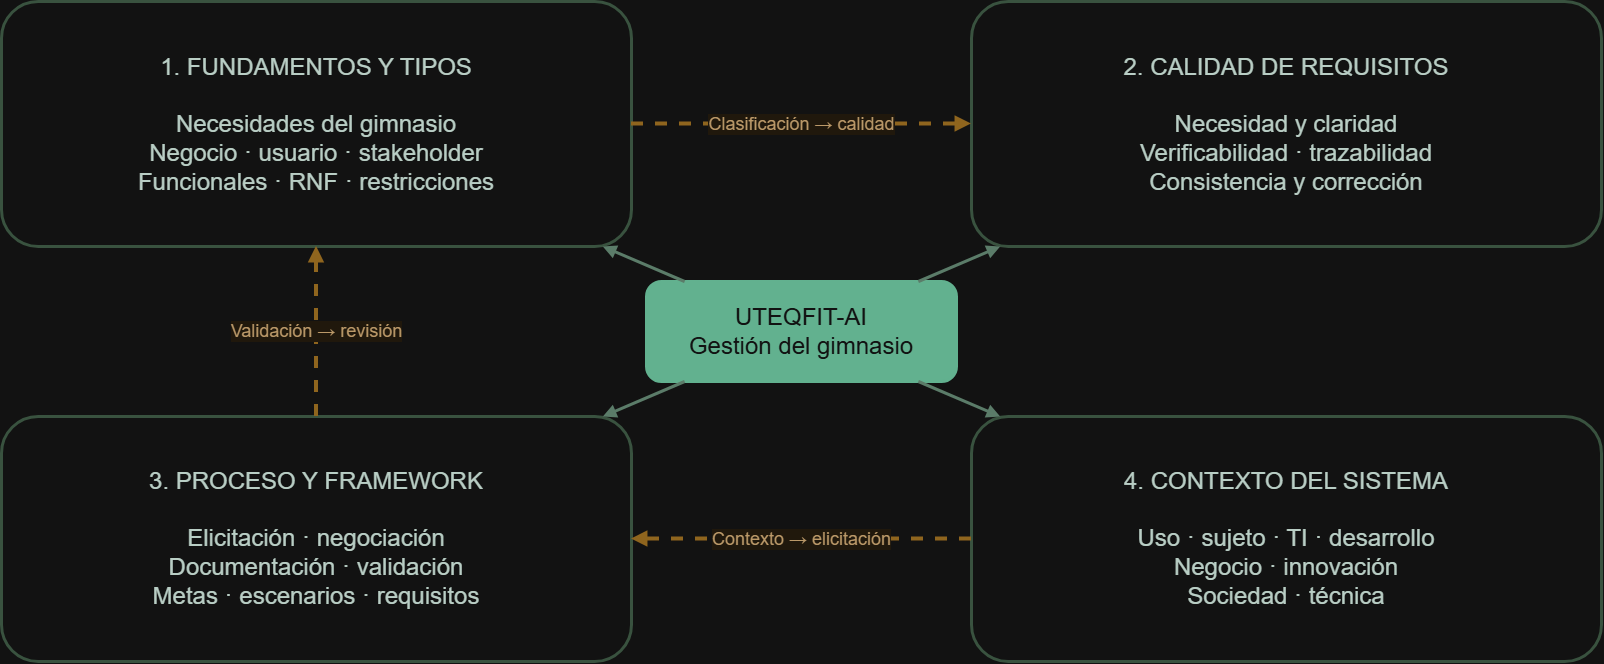
\includegraphics[width=\textwidth]{figuras/mapa_conceptual.png}
%   \caption{Mapa conceptual integrador de la unidad 1}
%   \label{fig:mapa}
% \end{figure}




% Conclusiones de la práctica experimental GA-SUM-01.
% Cada integrante debe redactar su propia conclusión de mínimo 80 palabras.

\section*{Conclusiones}
\addcontentsline{toc}{section}{Conclusiones}

\begin{enumerate}

\item \textbf{Conclusión de Luis Yépez}

Durante esta práctica comprendí que para desarrollar un sistema no basta con pensar en las funciones que tendrá. Primero debemos identificar las necesidades de los usuarios y conocer el contexto donde se utilizará. En el proyecto UteqFit-AI analizamos los tipos de requisitos, sus propiedades y las ocho perspectivas de contexto que presenta Pohl (2025)~\cite{pohl2025}. Esto nos permitió identificar aspectos importantes como el control de asistencias, la protección de los datos de los estudiantes y las posibles rutinas con inteligencia artificial. También aprendí que los requisitos deben ser claros, verificables y revisados con los responsables del gimnasio~\cite{ieee29148}. Considero que este trabajo nos ayudará a organizar mejor el proyecto y evitar problemas durante su desarrollo.

% Alan y Anderson agregarán aquí las otras cuatro conclusiones.

\end{enumerate}


% Se activa cuando Anderson exporte las fuentes de Zotero o Mendeley a referencias.bib
\bibliographystyle{IEEEtran}
\bibliography{referencias}

% Paso 2 c) y d) (Anderson).
\appendix
\section*{Anexos}
\addcontentsline{toc}{section}{Anexos}

\subsection*{Anexo A. Lista de referencias IEEE exportada}
\addcontentsline{toc}{subsection}{Anexo A. Lista de referencias IEEE exportada}
% Paso 2 c): la lista exportada desde Zotero o Mendeley.

\subsection*{Anexo B. Biblioteca en el gestor de referencias}
\addcontentsline{toc}{subsection}{Anexo B. Biblioteca en el gestor de referencias}
% Paso 2 d): captura de pantalla de la biblioteca. Guardarla en figuras/ y quitar el comentario.
% \begin{figure}[h]
%   \centering
%   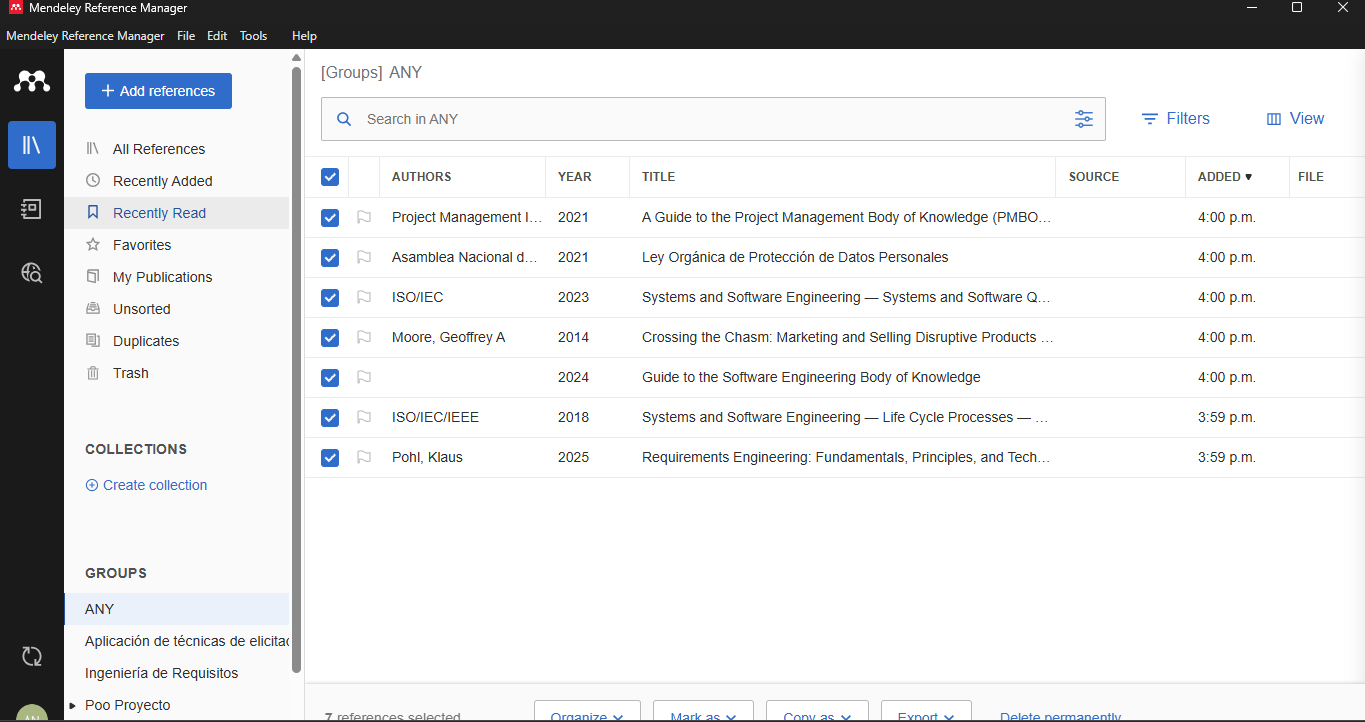
\includegraphics[width=\textwidth]{figuras/biblioteca_zotero.png}
%   \caption{Biblioteca de referencias en el gestor}
% \end{figure}


% Paso 6 d): la declaración de uso de IA va al final del documento.
% La escribe el grupo cuando el trabajo esté terminado.
\section*{Declaración de uso de IA}
\addcontentsline{toc}{section}{Declaración de uso de IA}

Usé ChatGPT-6.1-Sol para preparar el borrador de las secciones 2.1 y 2.2, organizar la bibliografía y redactar el límite y la visión de UteqFit-AI. Para adaptar esos apartados al gimnasio de la UTEQ, me basé en la tabla de requisitos que el equipo publicó en el repositorio.

\end{document}
